%%%%%%%%%%%%%%%%%%%%%%%%%%%%%%%%%%%%%%%%%%%%
% 
% Last edits: Nov 9, 2016
%%%%%%%%%%%%%%%%%%%%%%%%%%%%%%%%%%%%%%%%%%%%

\documentclass[12pt]{article}
\usepackage{natbib}
\usepackage[letterpaper, margin=1in]{geometry}
\usepackage{graphicx}
\usepackage[table,xcdraw]{xcolor}
\usepackage{wrapfig}
\usepackage{enumitem}
\setlist[enumerate]{itemsep=0mm}
\usepackage{multirow}
\usepackage{lscape}
\usepackage{caption}
\usepackage{subcaption}
\usepackage{float}
\usepackage{hyperref}
\usepackage{tabularx}
\usepackage{rotating}


\begin{document}
\noindent{Alexandra Pulwicki \\ \today}

\begin{center}
\Large \textbf{Results\\ Observations}
\end{center}


\section*{Overview}

This document shows an overview of the data that are available for the project. It provides a first look at the processed data and provides figures that visualize the data. Section 1 examines the density data and uncertainty and potential systematic errors associated with measurements made in the snowpits and using a Federal Sampler. Section 2 briefly looks at the snow depths measured at the study glaciers. Section 3 visualizes the collected zigzag data. Section 4 examines the various ways to estimate snow water equivalent (SWE) at each measurement location. It focuses on options for how to interpolate density measurements and then visualizes estimated SWE at the measurement locations. 


\tableofcontents
\pagebreak



%%%
\section{Density Estimates}
%%%

\subsection{Basic statistics}

The standard deviation of each type of density measurement is less than 10\% of the mean density (Table \ref{tab:density_stats}). For snowpit derived densities, the mean density is within one standard deviation between glaciers . The densities estimated using the Federal Sampler differed between glacier within one standard deviation. Our density measurements on Glacier 2 were lower than those on Glacier 4, while density measurements taken on Glacier 13 were the same as Both Glaciers 2 and 4. The mean of all Federal Sampler derived density values was skewed by the proportionally large number of measurements obtained on Glacier 13.

\begin{table}[h!]
\centering
\caption{Statistics of integrated densities measured using Federal Sampler or vertical density profiles (of snow wedge measurmenets) in snow pits. Mean, standard deviation (std), and number ($n$) of snow density (kg m$^{-3}$) measurements on study glaciers is shown.}
\label{tab:density_stats}
\begin{tabular}{c|ccc|ccc}
 & \multicolumn{3}{c}{\textbf{Snowpits}} & \multicolumn{3}{|c}{\textbf{Federal Sampler}} \\
\multirow{-2}{*}{\textbf{Glacier}} & Mean & Std & n & Mean & Std & n \\ \hline \hline
\textbf{Glacier 4} & 348 & 13 & 3 & 355 & 18 & 7 \\
\textbf{Glacier 2} & 333 & 26 & 4 & 286 & 34 & 7 \\
\textbf{Glacier 13} & 349 & 26 & 3 & 316 & 40 & 17 \\  \hline
\textbf{All} & 342 & 26 & 10 & 318 & 42 & 31
\end{tabular}
\end{table}

\subsection{Federal Sampler measurements and snow depth}
\label{sec:FSdensity&depth}

There is a positive linear relation (R$^2$ = 0.59, p$<$0.01) between measured snow density and depth for all Federal Sampler measurements (Figure \ref{fig:all_depth}). This positive relationship could be a result of physical processes, such as compaction, and/or artefacts during data collection; however, it seems more likely that this trend is a result of measurement artefacts for a number of reasons. First, the range of densities measured by the Federal sampler is large (225--410 kg m$^{-3}$) and the extreme values seem unlikely to exist at these study glaciers, which experience a continental snowpack with minimal mid-winter melt events. Previous unpublished density measurements taken on Glacier 2 range between 264 and 396 kg m$^{-3}$ for five study years with a maximum density difference of 110 kg m$^{-3}$ in any one year (Flowers, 2016, personal communication). Second, compaction effects would likely be small at these study glaciers because of the relatively shallow snowpack (deepest measurement was 340 cm). Third, no linear relationship exists between depth and snowpit-derived density (R$^2$ = 0.05) as can be seen in a plot of the depth-density relationship in snowpits in Figure \ref{fig:all_depth}. Together, these reasons lead us to conclude that the Federal Sampler measurements are biased. Linear detrending can correct the density data but it was decided to use uncorrected data for future analysis.



\begin{figure}[p]
	\centering
	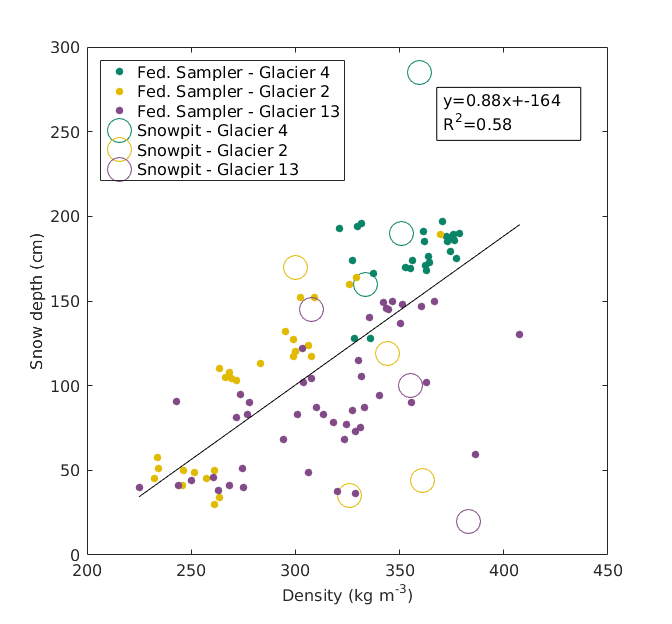
\includegraphics[width =0.85\textwidth]{DepthDensity_SWEonly.png}\\
	\caption{Relationship between measured density and snow depth for all Federal Sampler and snowpit locations. A linear regression of depth and density for Federal Sampler (FS) measurements is shown as a solid line and for snowpits (SP) is shown as a dashed line.}
	\label{fig:all_depth}
\end{figure}


\subsection{Density uncertainties}

\subsubsection{Snowpit densities}

Uncertainty in estimating density from snowpits stems from measurement errors and incorrect assignment of density to layers that could not be sampled (i.e. ice lenses and `hard' layers). To determine a possible range of snowpit-derived integrated snow density values, the original data are used and three quantities are varied. Ice layer density is varied between 700 and 900 kg m$^{-3}$, ice layer thickness is varied by $\pm$1 cm of the observed thickness, and the density of layers identified as being too hard to sample (but not ice) was varied between 600 and 700 kg m$^{-3}$. 

The range of integrated density values is always less than 15\% of the reference density, with the largest ranges present on Glacier 2 (Table \ref{tab:density_SP}). Density values for shallow pits that contained ice lenses were particularly sensitive to changes in density and ice lens thickness. 

\begin{sidewaystable}[]
\centering
\caption{Summary of reference and range of integrated snow density calculated from  snowpit measurements. The reference density values are calculated with an ice layer density of 917 kg m$^{-3}$ and a `hard' snow density of 600 kg m$^{-3}$. To determine the error in estimating integrated snow density, ice density, ice thickness, and the `hard' layer density are varied between 700 and 917 kg m$^{-3}$, $\pm$ 1 cm, and 500 and 600 kg m$^{-3}$, respectively.}
\label{tab:density_SP}
\resizebox{\textwidth}{!}{%
\begin{tabular}{lcccccccc}
\multirow{2}{*}{\textbf{Snowpit Name}} &  & \multicolumn{4}{c}{\textbf{Density (kg m$^{-3}$)}} &  \\
\multirow{-2}{*}{} & \multirow{-2}{*}{\textbf{Depth (m)}} & \textit{Reference} & \textit{Minimum} & \textit{Maximum} & \textit{Range} & \multirow{-2}{*}{\textbf{\begin{tabular}[c]{@{}c@{}}Range as \% \\ of reference value\end{tabular}}} & \multirow{-2}{*}{\textbf{\begin{tabular}[c]{@{}c@{}}Elevation\\ (m a.s.l)\end{tabular}}}& \multirow{-2}{*}{\textbf{\begin{tabular}[c]{@{}c@{}}Average \\ Temperature ($^{\circ}$) \end{tabular}}}\\ \hline \hline

Glacier 4, Lower & 190 & 350.9 & 343.2 & 359.1 & 15.9 & 4.5 & 2154 & $-$ 4.3\\
Glacier 4, Upper & 160 & 333.4 & 316.6 & 349.6 & 33.0 & 9.9  & 2298 & $-$ 5.7\\
Glacier 4, Accumulation& 285 & 359.7 & 356.6 & 362.4 & 5.8 & 1.6  & 2482 & $-$ 6.8\\  \hline
Glacier 2, Lower  & 44 & 360.9 & 328.6 & 377.3 & 48.7 & 13.5 & 2175 & $-$ 3.7 \\
Glacier 2, Zone 4A & 35 & 325.8 & 307.9 & 344.7 & 36.8 & 11.3 & 2261 & $-$ 3.4 \\
Glacier 2, Upper  & 119 & 344.0 & 327.1 & 361.9 & 34.8 & 10.1 & 2349 & $-$ 6.6 \\ 
Glacier 2, Accumulation & 170 & 300.2 & 298.6 & 303.1 & 4.5 & 1.5  & 2550 & $-$ 7.4\\  \hline
Glacier 13, Lower  & 20 & 383.0 & 383.0 & 383.0 & 0 & 0  & 2139 & $-$ 0.1\\
Glacier 13, Upper & 100 & 355.4 & 345.6 & 366.9 & 21.3 & 6.0 & 2257 & $-$ 1.7 \\
Glacier 13, Accumulation & 145 & 307.8 & 306.4 & 308.2 & 1.8 & 0.6 & 2521 & $-$ 5.6
\end{tabular}%
}
\end{sidewaystable}

\subsubsection{Federal Sampler densities}

Mean Federal Sampler derived density has a larger range of values over the study glaciers when compared to snowpit densities (Table \ref{tab:density_TubeRange}). The percent range is also larger than snowpit densities for many of the measurement locations. 

\begin{table}[]
\centering
\caption{Range of densities estimated from Federal Sampler measurements. The number ($n$) of reliable measurements, as well as the minimum, maximum, and mean density are shown. The density range, given as a percent of the mean density, is also shown. Location refers to the snowpit name as shown in Figure ??}
\label{tab:density_TubeRange}
\begin{tabular}{lcccccc}
\multicolumn{1}{c}{\multirow{2}{*}{\textbf{Location}}} & \multirow{2}{*}{\textbf{$n$}} & \multicolumn{3}{c}{\textbf{Density (kg m$^{-3}$)}} & \multirow{2}{*}{\textbf{\begin{tabular}[c]{@{}c@{}}Range as \%\\ of mean (\%)\end{tabular}}}& \multirow{2}{*}{\textbf{\begin{tabular}[c]{@{}c@{}}Elevation\\ (m a.s.l)\end{tabular}}} \\
\multicolumn{1}{c}{} &  & Mean & Minimum & Maximum &  \\ \hline  \hline
G04\_Z3A\_SWE & 3 & 334 & 309 & 358 & 14 & 2229 \\
G04\_USP & 6 & 311 & 274 & 353 & 22 & 2298 \\
G04\_Z2A\_SWE & 3 & 360 & 303 & 431 & 35 & 2162 \\
G04\_LSP & 7 & 272 & 250 & 297 & 13 & 2154 \\
G04\_Z5B\_SWE & 2 & 337 & 324 & 350 & 7  & 2360\\
G04\_Z5A\_SWE & 3 & 311 & 275 & 351 & 21  & 2328\\
G04\_Z5C\_SWE & 2 & 361 & 350 & 373 & 6  & 2332\\  \hline
G02\_Z5C\_SWE & 2 & 296 & 245 & 347 & 28 & 2332 \\
G02\_USP & 7 & 294 & 232 & 353 & 34  & 2349\\
G02\_Z7A\_SWE & 3 & 326 & 304 & 349 & 12  & 2403\\
G02\_Z7B\_SWE & 2 & 336 & 320 & 351 & 9 & 2458 \\
G02\_Z7C\_SWE & 3 & 351 & 338 & 365 & 7 & 2442 \\
G02\_Z3B\_SWE & 3 & 349 & 341 & 353 & 3  & 2172\\
G02\_LSP\_SWE & 7 & 331 & 302 & 349 & 13 & 2175 \\ \hline
G13\_ASP & 8 & 343 & 277 & 395 & 33  & 2521\\
G13\_651 & 3 & 329 & 318 & 345 & 7  & 2574\\
G13\_652 & 2 & 319 & 291 & 346 & 15  & 2542\\
G13\_654 & 3 & 298 & 266 & 318 & 14  & 2571\\
G13\_655 & 1 & 300 &-- & -- & --  & 2561\\
G13\_656 & 3 & 279 & 227 & 315 & 24  & 2541\\
G13\_657 & 3 & 331 & 323 & 338 & 4  & 2483\\
G13\_658 & 2 & 343 & 333 & 354 & 6  & 2427\\
G13\_659 & 3 & 245 & 232 & 258 & 7 & 2327 \\
G13\_Z7C\_SWE & 2 & 270 & 253 & 287 & 9  & 2297\\
G13\_USP & 6 & 294 & 247 & 359 & 31  & 2258\\
G13\_Z4C\_SWE & 4 & 342 & 334 & 350 & 5 & 2206 \\
G13\_744 & 3 & 323 & 298 & 347 & 14 & 2210 \\
G13\_Z3B\_SWE & 3 & 333 & 308 & 351 & 12 & 2156 \\
G13\_Z4B\_SWE & 2 & 332 & 312 & 351 & 11  & 2214\\
G13\_Z5A\_SWE & 3 & 276 & 240 & 301 & 17  & 2271\\
G13\_Z5B\_SWE & 2 & 255 & 254 & 257 & 1 & 2226
\end{tabular}
\end{table}

\subsection{Comparing density from snowpit and Federal Sampler measurements}

To compare snowpit-derived densities and Federal Sampler-derived densities, eight Federal Sampler measurements were taken around two snowpit locations on each study glacier.  The overall range of Federal Sampler-derived densities is larger than that of the snowpit-derived density values (Figure \ref{fig:density_pitVStube}). Within the minimum and maximum snowpit-derived densities, the values are indistinguishable for all snowpit locations, except for the accumulation snowpit on Galcier 13 (`G13\_ASP').

\begin{figure}[H]
	\centering
	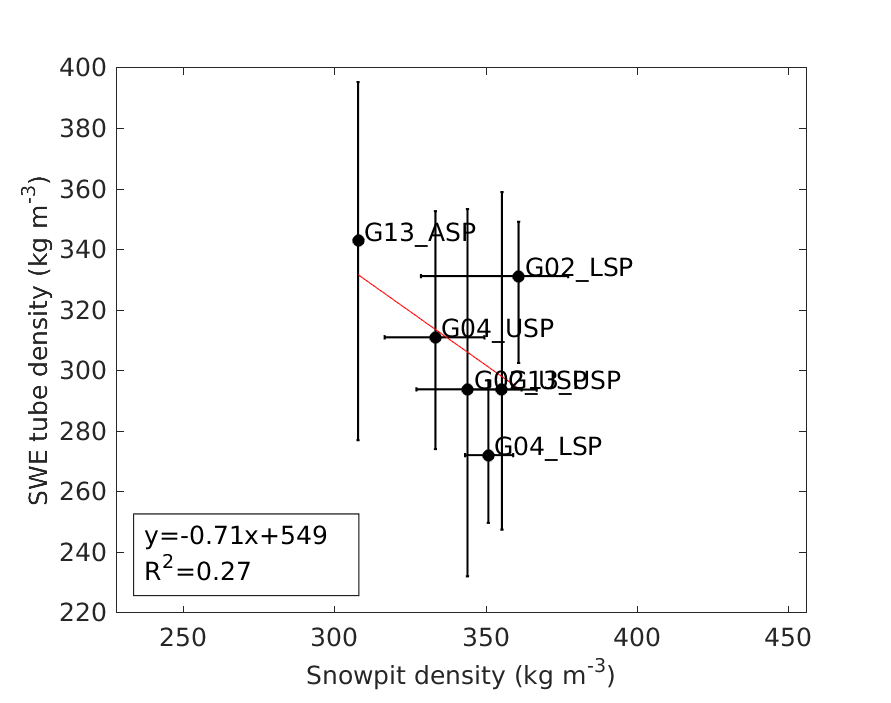
\includegraphics[width =0.95\textwidth]{SnowpitVsSWEtube_all.png}\\
	\caption{Comparison of integrated density estimated using wedge cutters in a snowpit and density estimated using Federal Sampler measurements for Glacier 4 (G04), Glacier 2 (G02) and Glacier 13 (G13). Error bars are minimum and maximum values for each estimate as reported in Table \ref{tab:density_SP} and \ref{tab:density_TubeRange}. }
	\label{fig:density_pitVStube}
\end{figure}


\subsection{Density and elevation}

A linear regression of density on topographic parameters is often used to interpolate density values between measurement locations \citep[e.g.][]{Elder1998, Molotch2005,Wetlaufer2016}. Since the density measurement locations spanned a large portion of the elevation range for each glacier, the density values are regressed on elevation only. Regression slopes differ in both magnitude and sign between snowpit-derived and Federal Sampler-derived densities (Table \ref{tab:elev_regress}). 

Snowpit-derived density decreases with elevation on Glaciers 2 and 13 and does not change with elevation on Glacier 4 (Figure \ref{fig:elev_snowpit}). The lower elevation sites on Glaciers 2 and 13 could have been melt affected. Warmer mean snow temperatures at the lower sites (Table \ref{tab:density_SP}) indicate that melt has occurred, which would increase snow density. Glacier 4 was probably not affect by melt, as snow temperatures are cool at all snowpit sites. 

Opposite relationship are seen in the regression of Federal Sampler-derived densities and elevation (Figure \ref{fig:elev_tube}). Density increases with elevation on Glacier 2 and there is no relationship with elevation on Glacier 4 and 13. The is a positive relationship between snow density and snow depth (Section \ref{sec:FSdensity&depth}) and a positive relationship between snow depth and elevation (Figure \ref{fig:depth_elev}) on Glacier 2, which results in a positive relationship between snow density and elevation. Since there is no significant relationship between snow depth and elevation on Glaciers 4 and 13, there is no relationship between snow density and elevation. 


\begin{table}[]
\centering
\caption{Summary of linear regressions between integrated density and elevation (m a.s.l.). }
\label{tab:elev_regress}
\begin{tabular}{lrrcrcc}
\multicolumn{1}{c}{\multirow{2}{*}{\textbf{Location}}} & \multicolumn{3}{c}{\textbf{\begin{tabular}[c]{@{}c@{}}Snowpit \\ Regression\end{tabular}}} & \multicolumn{3}{c}{\textbf{\begin{tabular}[c]{@{}c@{}}Fed. Sampler\\ Regression\end{tabular}}} \\
\multicolumn{1}{c}{} & \multicolumn{1}{c}{Equation} & \multicolumn{1}{c}{R$^2$} & \multicolumn{1}{l}{$n$} & \multicolumn{1}{c}{Equation} & R$^2$ & \multicolumn{1}{l}{$n$} \\ \hline \hline
Glacier 4 & 0.03$z+$274 & 0.16 & 3 & $-$0.16$z+$714 & 0.53 & 7 \\
Glacier 2 & $-$0.14$z+$659 & 0.75 & 4 & 0.24$z-$282 & 0.72 & 7 \\
Glacier 13 & $-$0.20$z+$802 & $>$0.99 & 3 & 0.12$z+$33 & 0.21 & 17 \\ \hline
All & $-$0.12$z+$618 & 0.50 & 10 & $-$0.14$z+$659 & 0.75 & 31
\end{tabular}
\end{table}


\begin{figure}[H]
  \makebox[\textwidth][c]{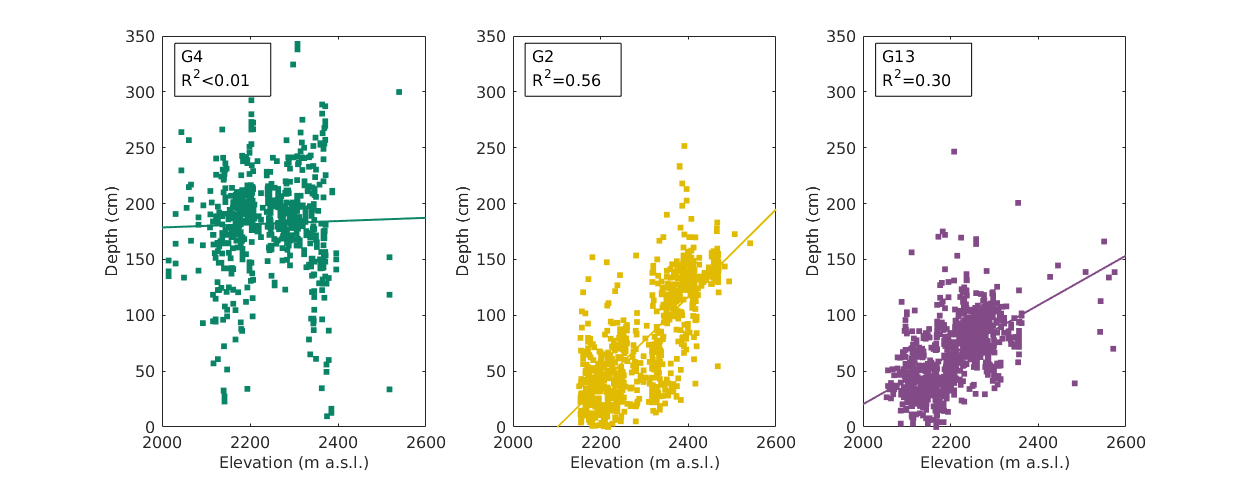
\includegraphics[width=1.2\textwidth]{DepthElevation.png}}%
	\caption{Relationship between measured snow depth and elevation at all sampling locations.}
	\label{fig:depth_elev}
\end{figure}


\begin{figure}[H]
	\centering
	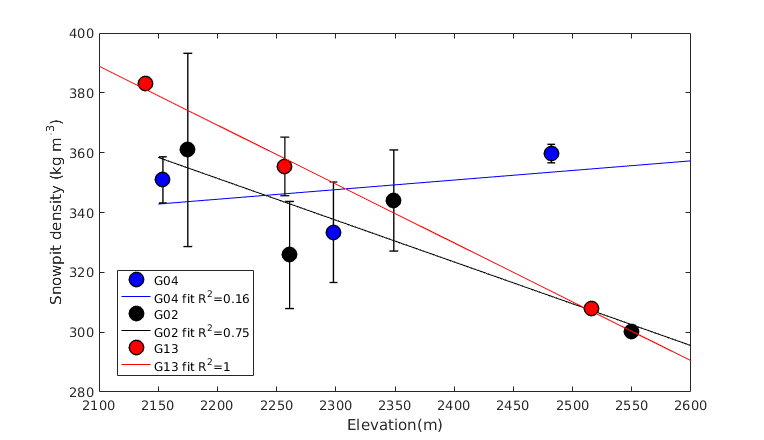
\includegraphics[width = 0.7\textwidth]{ElevationVsSnowpit_all.png}\\
	\caption{Relationship between snowpit-derived density and elevation for all study glaciers.}
	\label{fig:elev_snowpit}
\end{figure}


\begin{figure}[H]
	\centering
	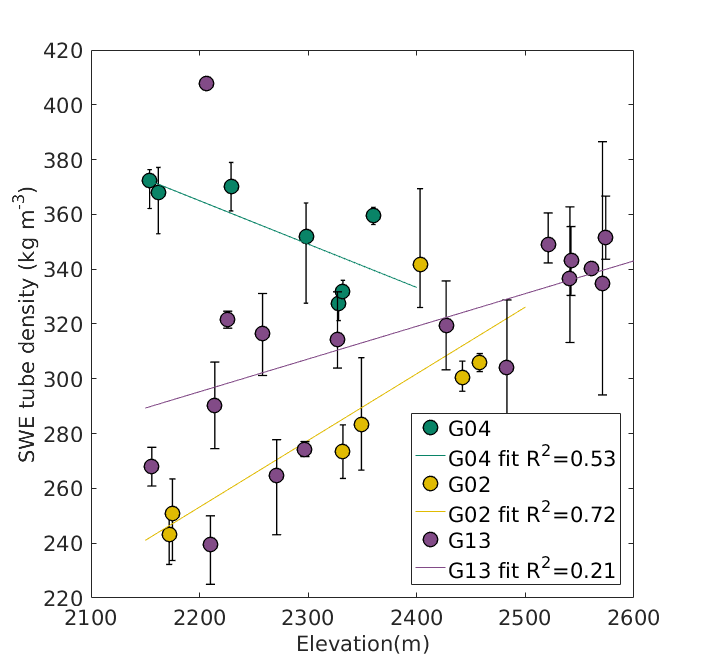
\includegraphics[width = 0.6\textwidth]{ElevationVsSWEtube_all.png}\\
	\caption{Relationship between Federal Sampler-derived density and elevation for all study glaciers.}
	\label{fig:elev_tube}
\end{figure}


\pagebreak

%%%%%%%%%%%%%%%%%%%%%%%%%%%%%%%%%%%%%%
\section{Linear and curvilinear transect snow depth data}

\begin{figure}[H]
    \centering
    \begin{subfigure}[b]{0.48\textwidth}
        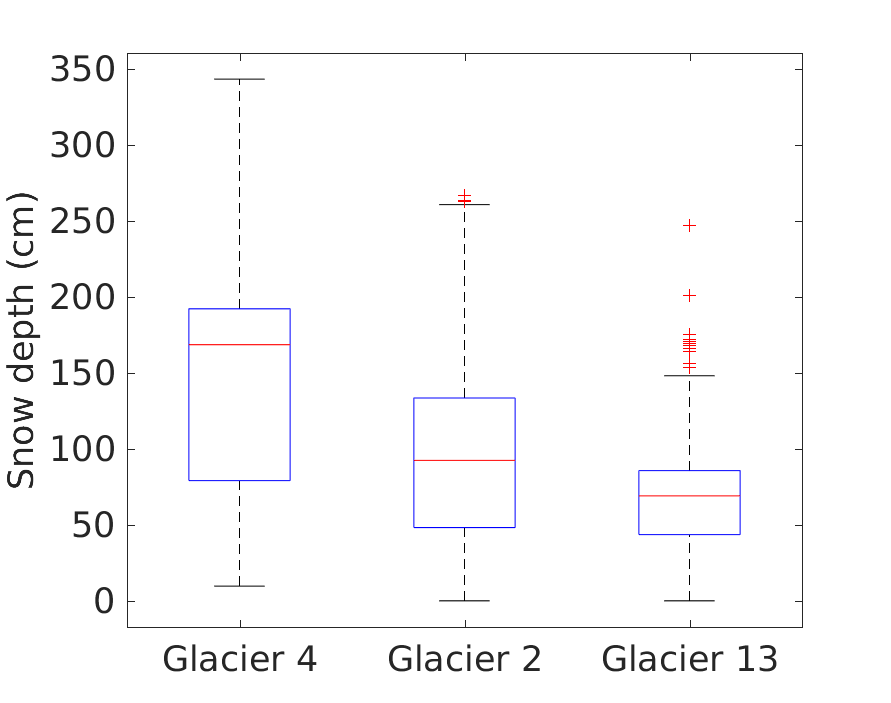
\includegraphics[width=\textwidth]{box_depth_wZZ.png}
        \caption{ }
        \label{fig:box_depth_wZZ}
    \end{subfigure}
    ~
    \begin{subfigure}[b]{0.48\textwidth}
        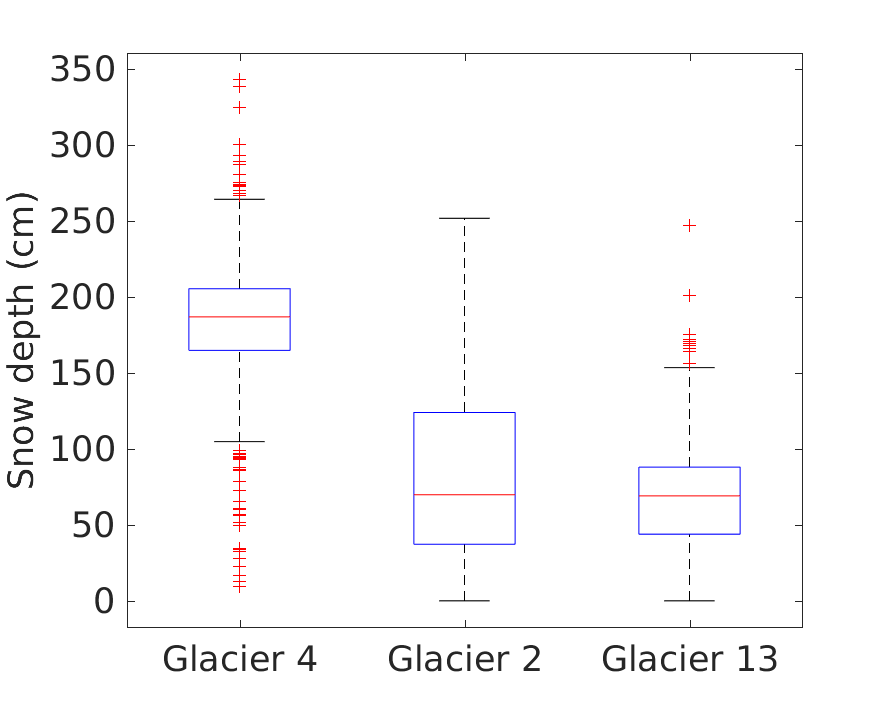
\includegraphics[width=\textwidth]{box_depth_noZZ.png}
        \caption{}
        \label{fig:box_depth_noZZ}
    \end{subfigure}

    \caption{Boxplots of snow depth measured on study glaciers. All snow depth values shown in (a) and snow depth values only from transects (zigzag, snowpit and Federal Sampler measurements excluded) shown in (b). Red line indicates median, blue box shows first quantiles, bars indicate minimum and maximum values (excluding outliers), and red crosses show outliers, which are defined as being outside of the range of 1.5 times the quartiles (approximately $\pm2.7\sigma$).}
    \label{fig:box_depth}
\end{figure}

Glacier 4 has the largest median and range of snow depth values, while Glacier 13 has the smallest (Figure \ref{fig:box_depth}). The boxplot of snow depth on Glacier 4 has different characteristics when only transect data is plotted (zigzag, snowpit and Federal Sampler measurements excluded). The range and IQR are smaller and there are significantly more points that are considered outliers. 

\pagebreak
%%%%%%%%%%%%%%%%%%%%%%%%%%%%%%%%%%%%%%
\section{Zigzag snow depth data}

A comparison of measured snow depth for each zigzag is shown in Figure \ref{fig:ZZ_boxplot}. The zigzags on Glacier 4 show minimal variability with a small range of values observed and few outliers. The mean depth is significantly larger at the highest elevation zigzag. Zigzags on Glacier 2 show more variability. The range on the middle elevation is the largest of all the zigzags measured and the highest zigzag has many outliers. The zigzags on Glacier 13 do not vary considerably in range, although the lower zigzags show a large number of outliers which may be a result of these locations being close to a supraglacial meltwater channel. 

The depths measured in each zigzag are shown in Figures \ref{fig:ZZ_G04}, \ref{fig:ZZ_G02}, and \ref{fig:ZZ_G13}. There is considerable variability both between zigzags and within each zigzag. For example, snow depths in G04\_Z5B are more uniform than in G04\_Z3A (Figure \ref{fig:ZZ_G04}). 

\begin{figure}[H]
	\centering
	 \makebox[\textwidth][c]{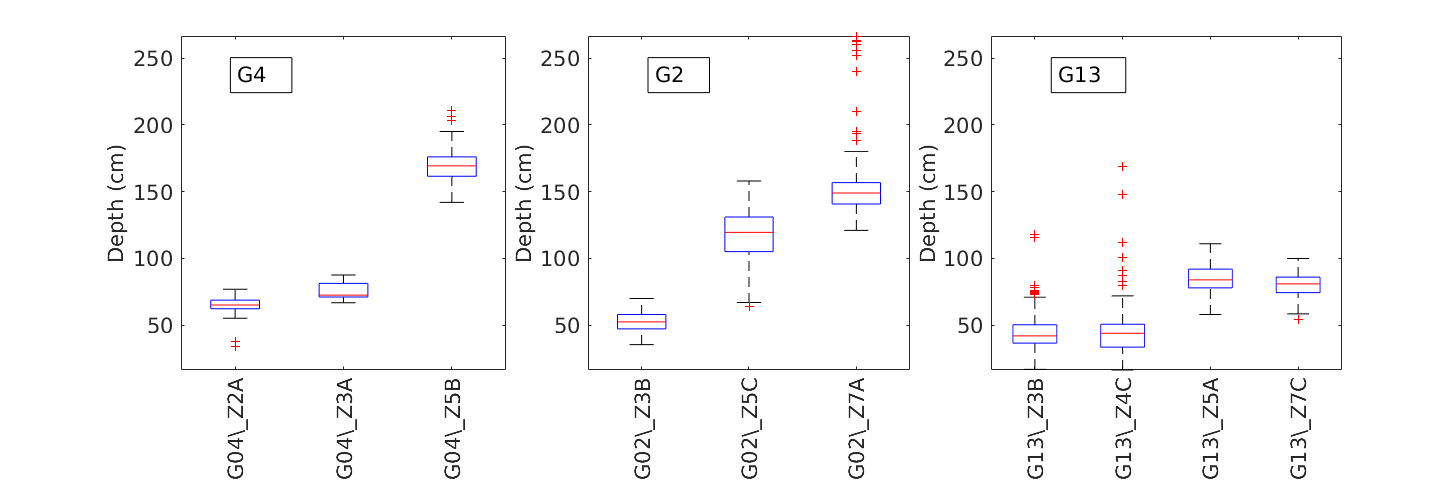
\includegraphics[width = 1.1\textwidth]{Zigzag_Boxplot.png}}%
	\caption{Boxplots of snow depth data measured at each zigzag location. See Figure \ref{fig:ZZ_locations} for locations of each zigzag.}
	\label{fig:ZZ_boxplot}
\end{figure}


\begin{figure}[H]
	\centering
	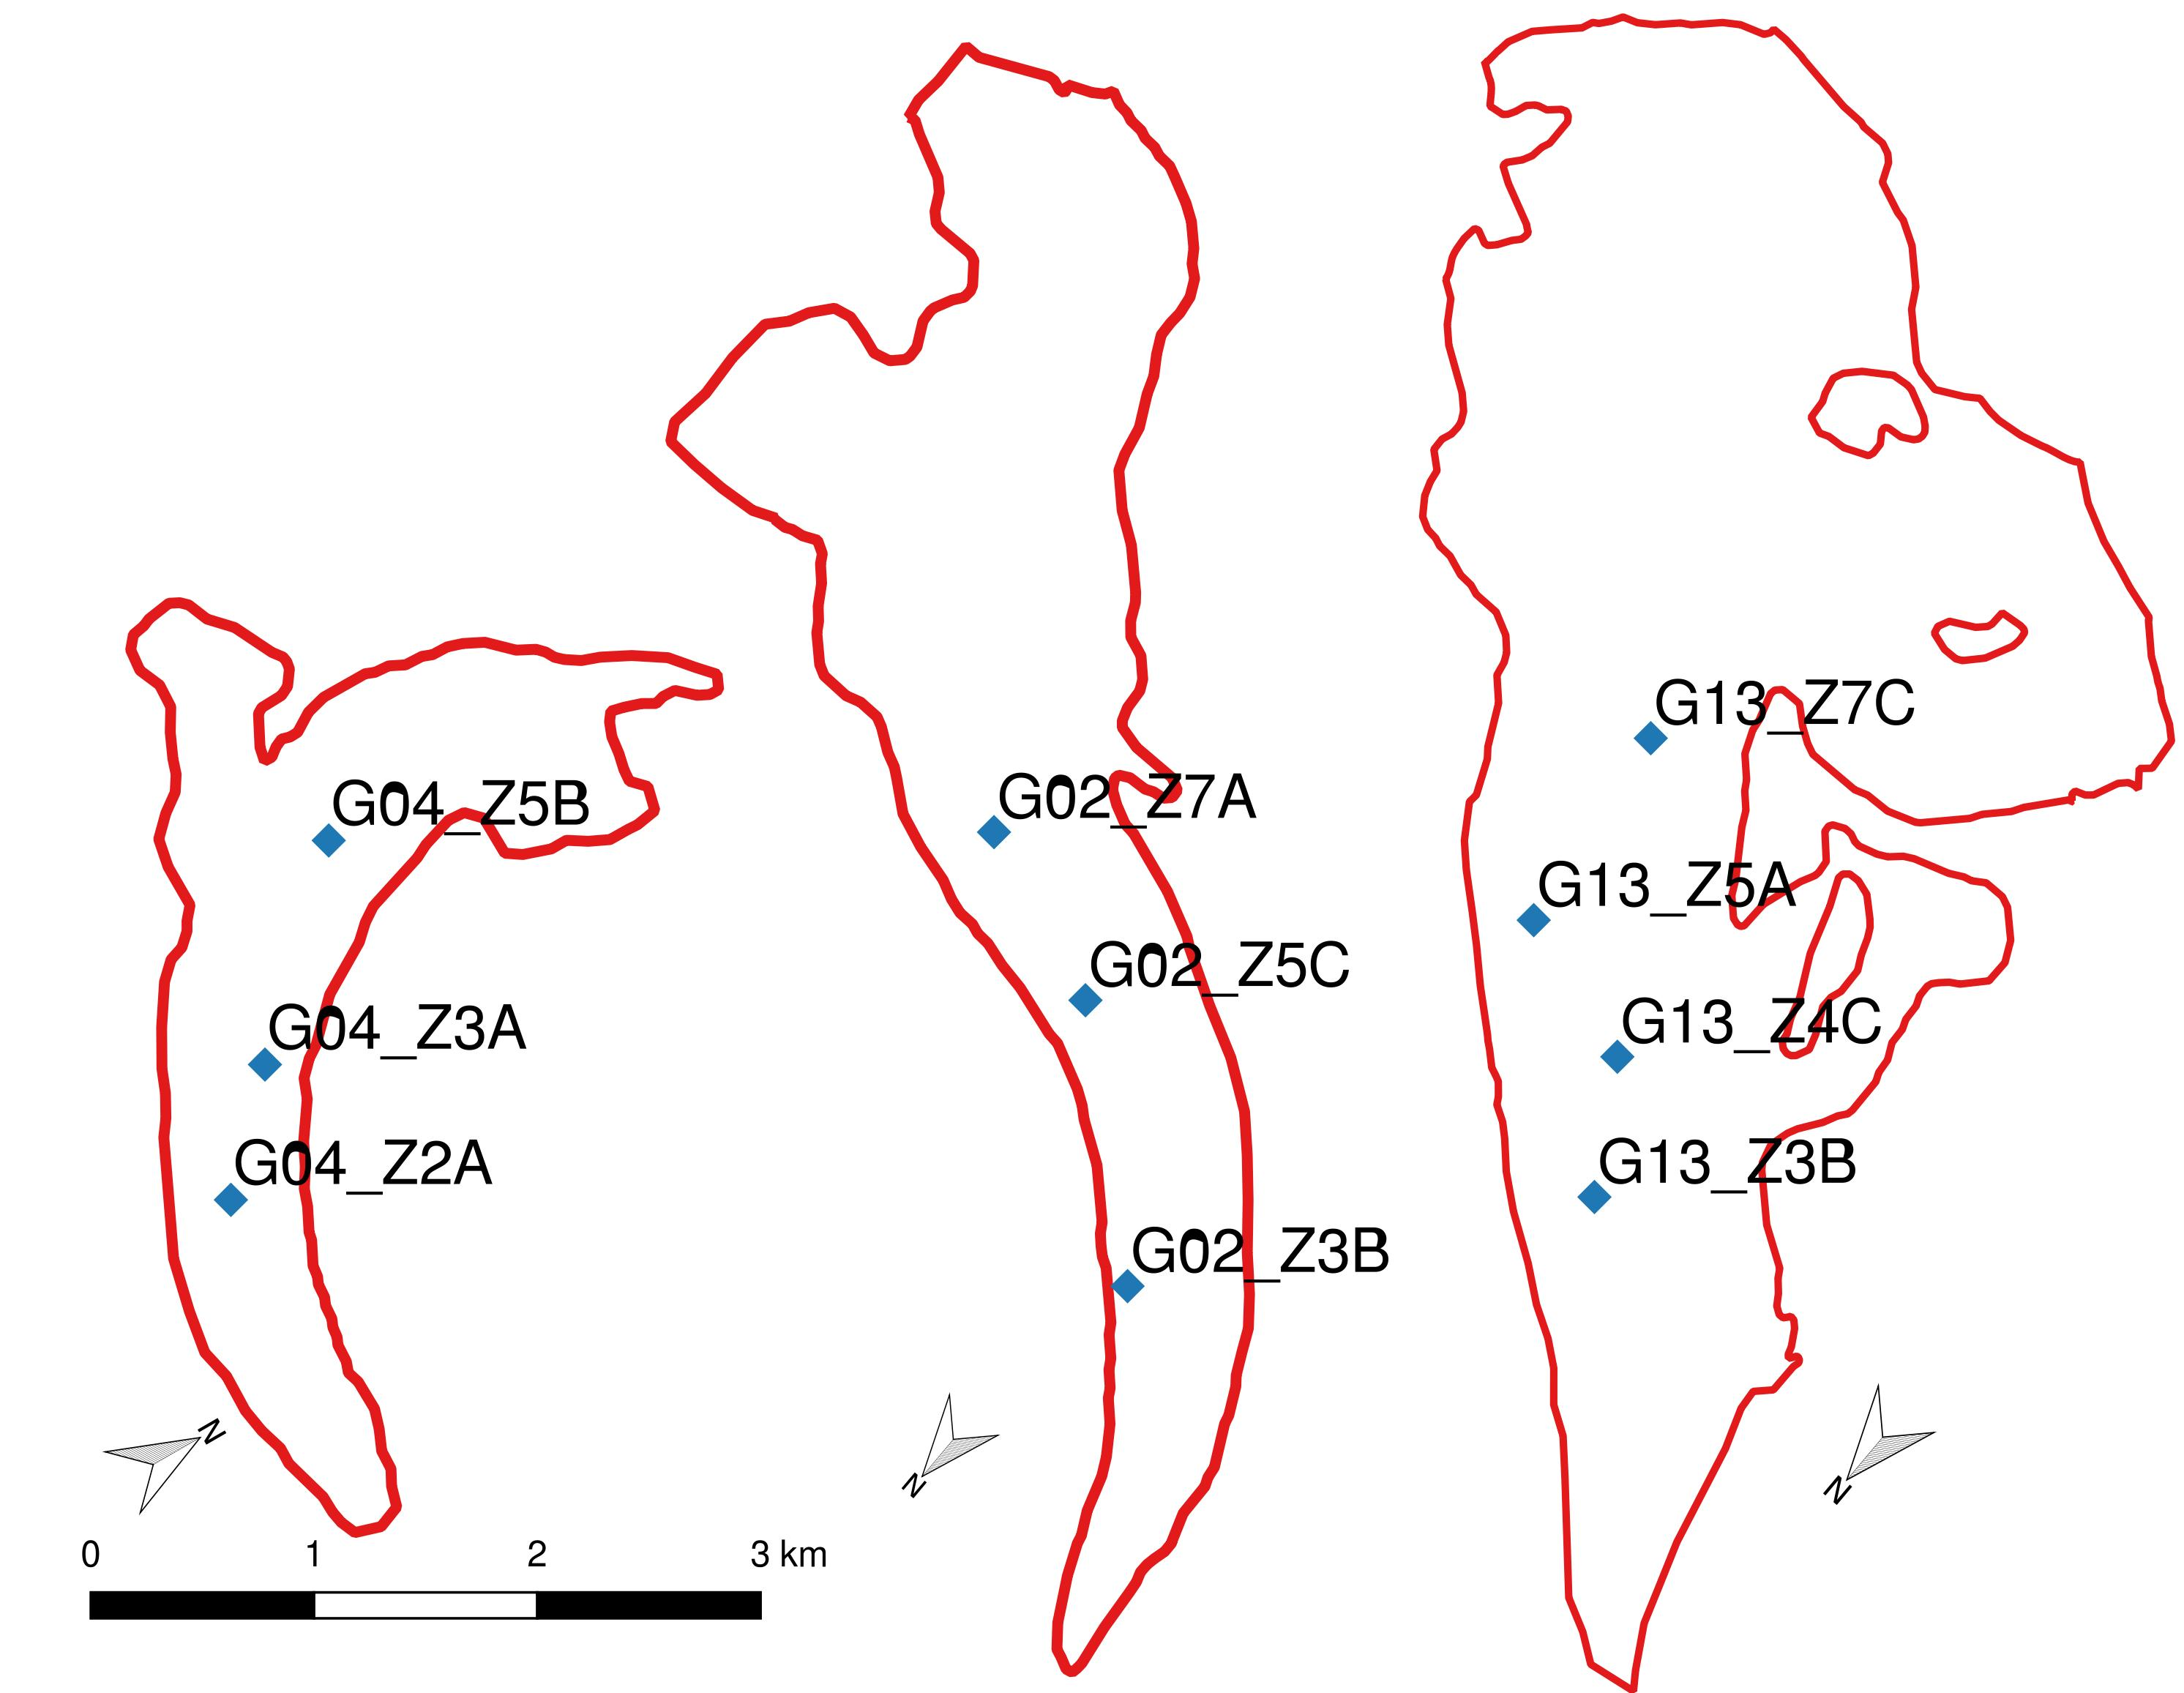
\includegraphics[width = 0.55\textwidth]{map_zigzaglocation_all.jpeg}\\
	\caption{Map of zigzag locations on Glaciers 4, 2 and 13 (left to right).}
	\label{fig:ZZ_locations}
\end{figure}

\begin{landscape}
\begin{figure}
	\centering
	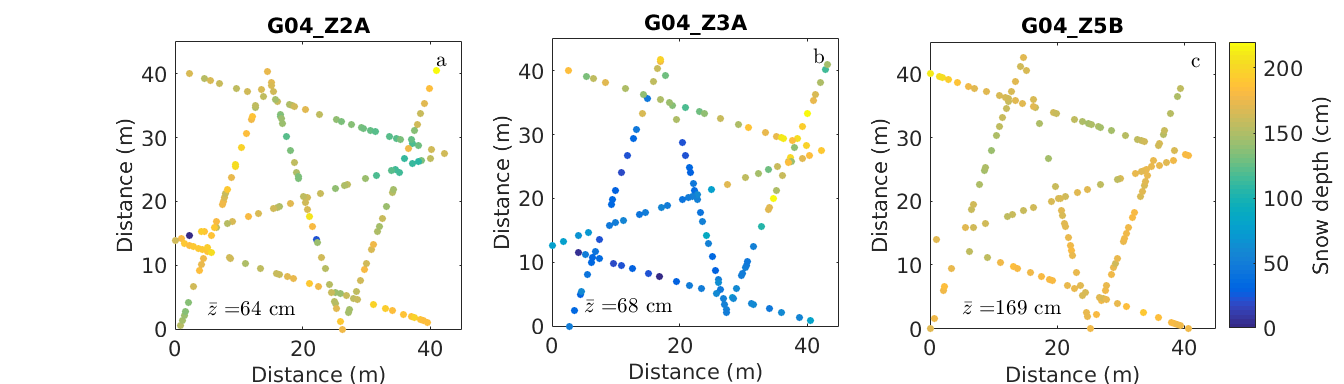
\includegraphics[width = 23 cm]{ZigzagDepth_G04.png}\\
	\caption{Snow depths measured in zigzags on Glacier 4. Mean depth ($\bar{z}$) is also reported. Zigzag elevations (left to right) are 2162, 2229 and 2360 m a.s.l. See Figure \ref{fig:ZZ_locations} for locations of each zigzag.}
	\label{fig:ZZ_G04}
\end{figure}

\begin{figure}
	\centering
	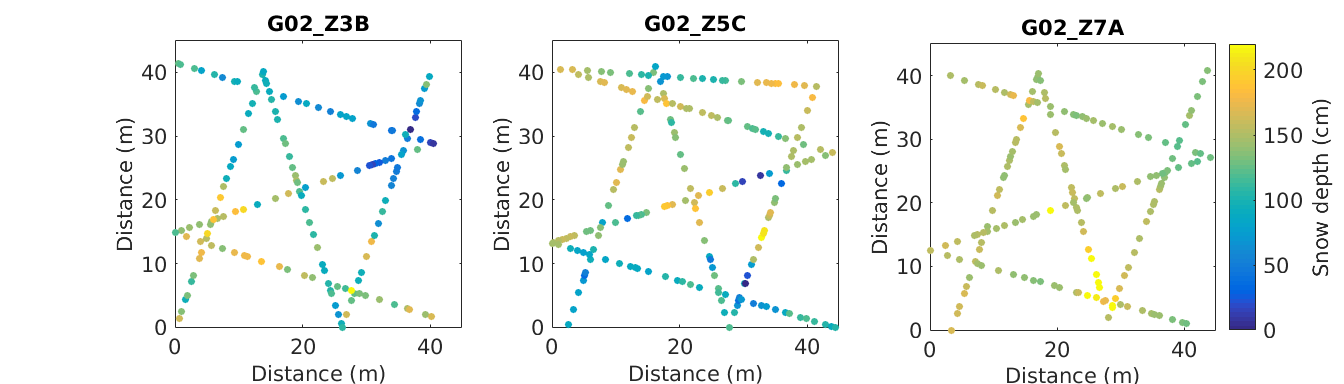
\includegraphics[width = 23 cm]{ZigzagDepth_G02.png}\\
	\caption{Snow depths measured in  zigzags on Glacier 2. Mean depth ($\bar{z}$) is also reported. Zigzag elevations (left to right) are 2172, 2332 and 2403 m a.s.l. See Figure \ref{fig:ZZ_locations} for locations of each zigzag.}
	\label{fig:ZZ_G02}
\end{figure}
\end{landscape}

\begin{figure}[H] 
	\centering
	 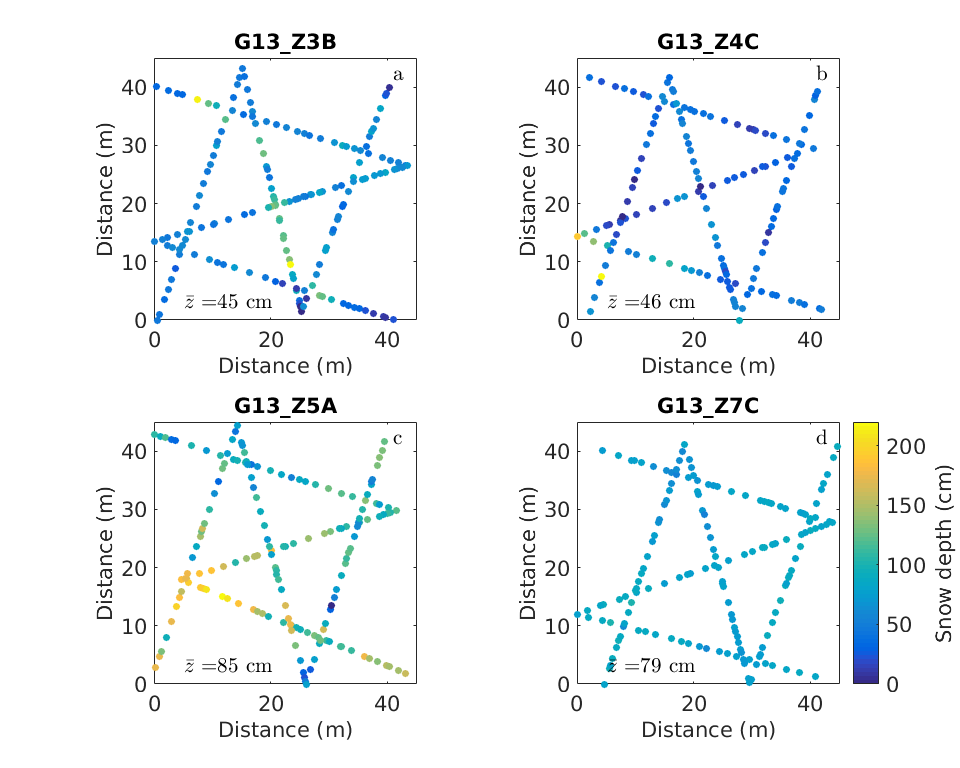
\includegraphics[width=0.9\textwidth]{ZigzagDepth_G13.png}%
	\caption{Snow depths measured in zigzags on Glacier 13. Mean depth ($\bar{z}$) is also reported. Zigzag elevations (a-d) are 2156, 2206, 2271 and 2297 m a.s.l. See Figure \ref{fig:ZZ_locations} for locations of each zigzag.}
	\label{fig:ZZ_G13}
\end{figure}


%%%%%%%%%%%%%%%%%%%%%%%%%%%%%%%%%%%%%%
\section{Snow water equivalent (SWE)}

Snow water equivalent (SWE) estimated for each sampling location can be seen in Figures  \ref{fig:SWEmap_S1} to \ref{fig:SWEmap_F4}. For maps of SWE calculated for each density option see the Appendix. Generally, SWE is highest on Glacier 4 and lowest on Glacier 13. Glacier 4 also shows considerable SWE variability within the basin, with both high and low values seen along a single transect. Note that the individual measurement locations overlap on the figure.

\begin{figure}[H]
	\centering
	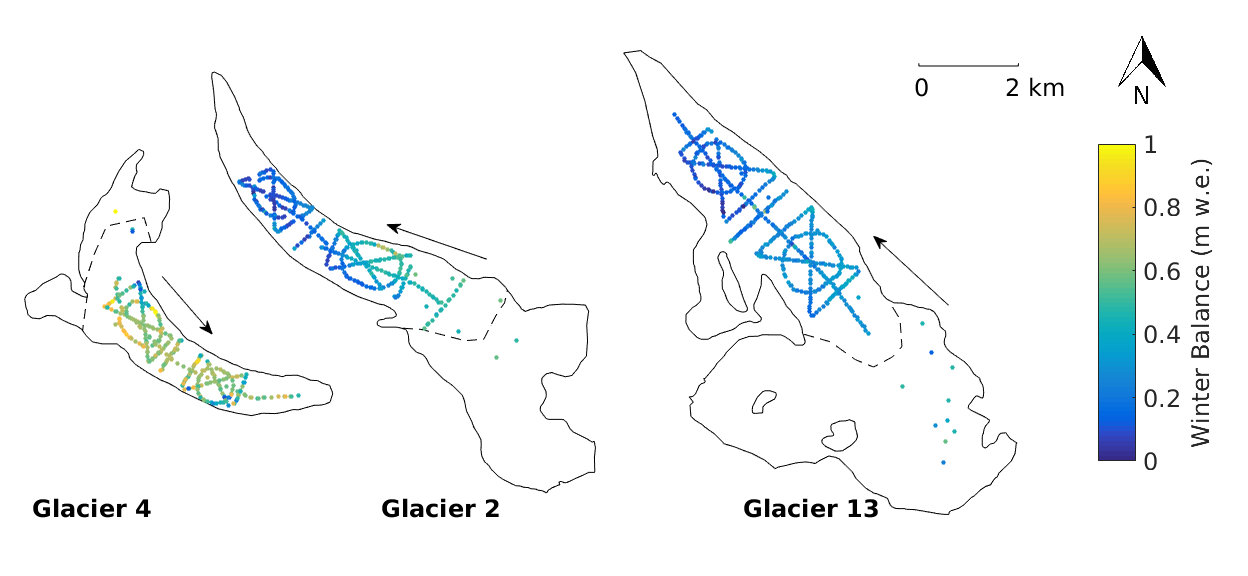
\includegraphics[width = \textwidth]{SWEmap_opt2.png}\\
	\caption{Estimated snow water equivalent (SWE) at measurement locations. Density was taken to be the mean value of all snowpit-derived densities (S1). Arrow shows ice flow direction.}
	\label{fig:SWEmap_S1}
\end{figure}

\begin{figure}[H]
	\centering
	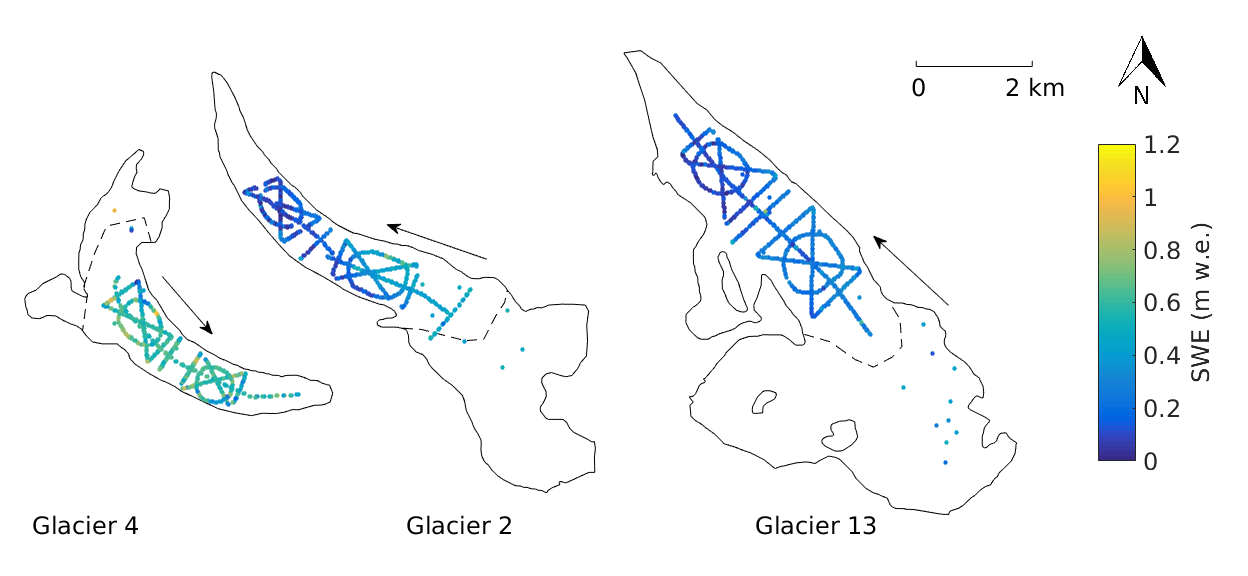
\includegraphics[width = \textwidth]{SWEmap_opt3.png}\\
	\caption{Estimated snow water equivalent (SWE) at measurement locations. Density was taken to be the mean value of all snowpit-derived densities (F1). Arrow shows ice flow direction.}
	\label{fig:SWEmap_F1}
\end{figure}

\begin{figure}[H]
	\centering
	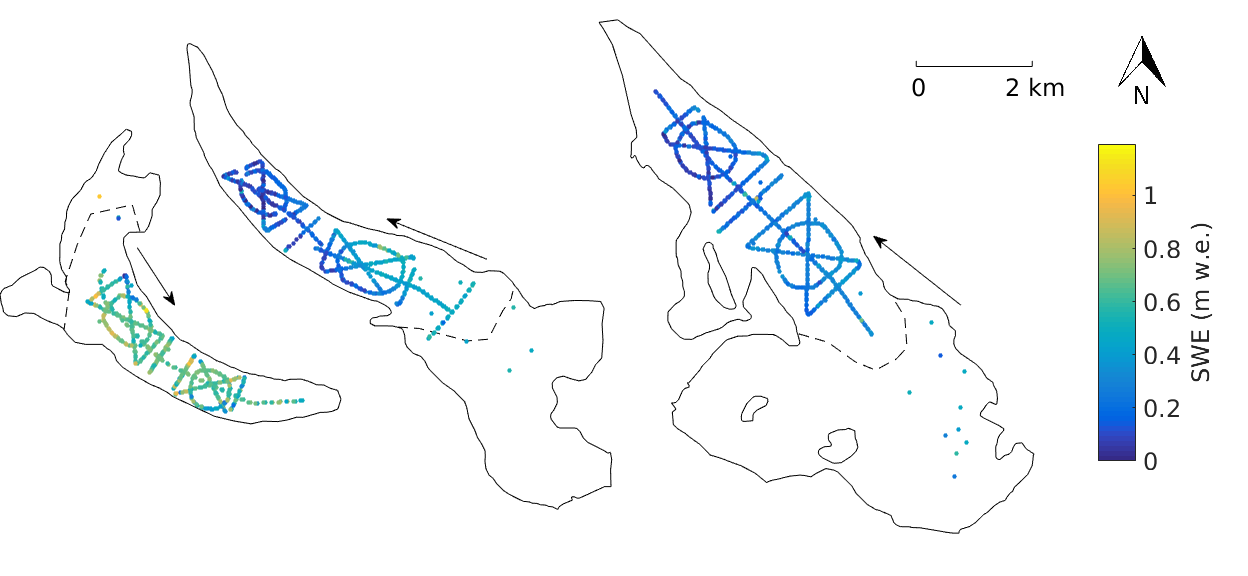
\includegraphics[width =\textwidth]{SWEmap_opt4.png}\\
	\caption{Estimated snow water equivalent (SWE) at measurement locations. Density was taken to be the mean value of snowpit-derived densities for each glacier (S2). Arrow shows ice flow direction.}
	\label{fig:SWEmap_S2}
\end{figure}

\begin{figure}[H]
	\centering
	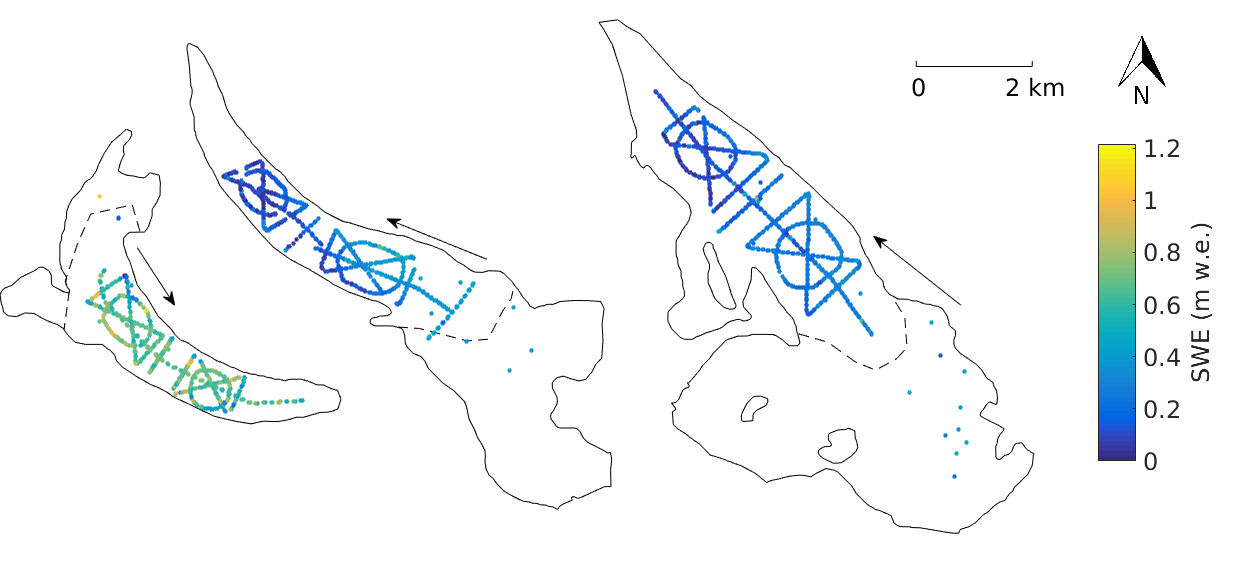
\includegraphics[width = \textwidth]{SWEmap_opt5.png}\\
	\caption{Estimated snow water equivalent (SWE) at measurement locations. Density was taken to be the mean value of Federal Sampler-derived densities for each glacier (F2). Arrow shows ice flow direction.}
	\label{fig:SWEmap_F2}
\end{figure}

\begin{figure}[H]
	\centering
	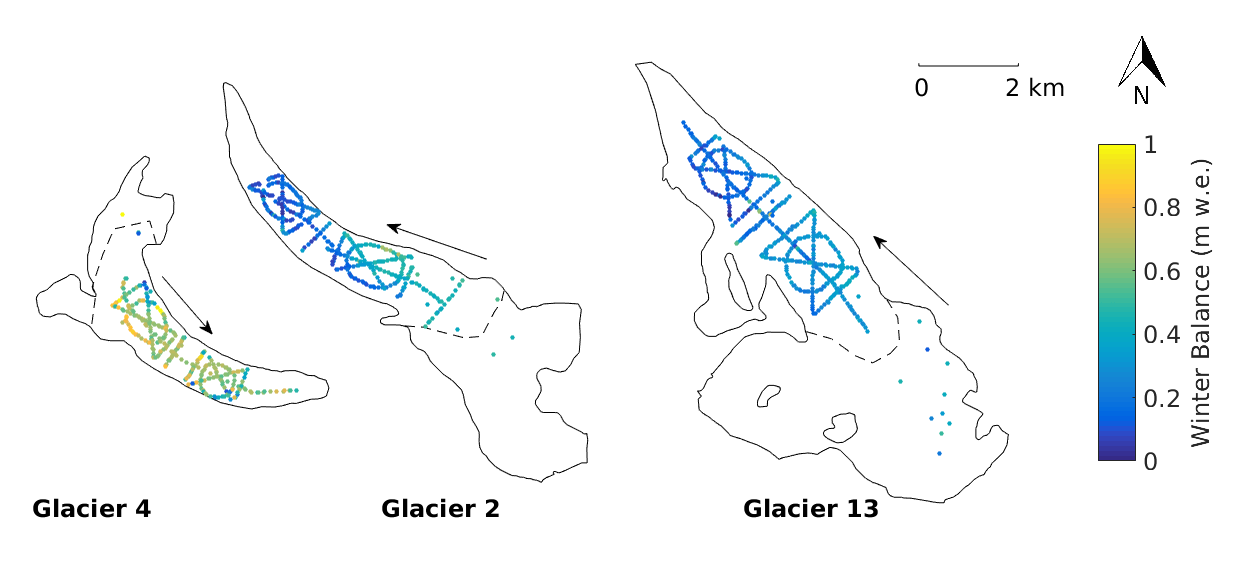
\includegraphics[width = \textwidth]{SWEmap_opt6.png}\\
	\caption{Estimated snow water equivalent (SWE) at measurement locations. Density was determined by using a linear fit between snowpit-derived density and elevation for each glacier (S3). Arrow shows ice flow direction.}
	\label{fig:SWEmap_S3}
\end{figure}

\begin{figure}[H]
	\centering
	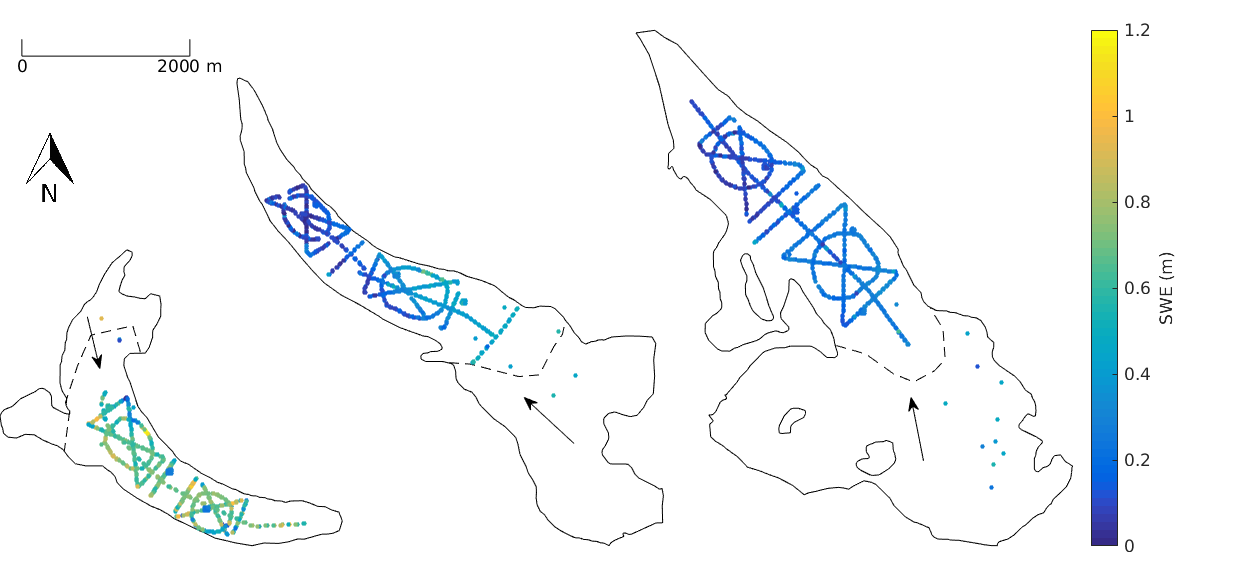
\includegraphics[width = \textwidth]{SWEmap_opt7.png}\\
	\caption{Estimated snow water equivalent (SWE) at measurement locations.Density was determined by using a linear fit between Federal Sampler-derived density and elevation for each glacier (F3). Arrow shows ice flow direction.}
	\label{fig:SWEmap_F3}
\end{figure}

\begin{figure}[H]
	\centering
	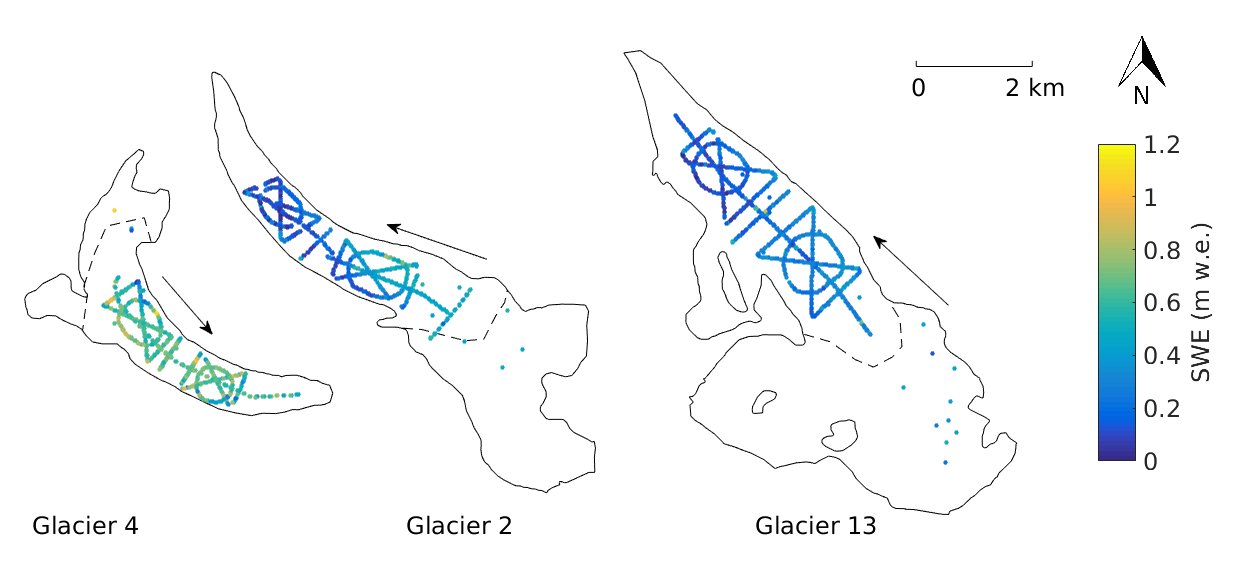
\includegraphics[width = \textwidth]{SWEmap_opt8.png}\\
	\caption{Estimated snow water equivalent (SWE) at measurement locations. Density was calculated using inverse distance weighting using all snowpit-derived densities (S4). Arrow shows ice flow direction.}
	\label{fig:SWEmap_S4}
\end{figure}

\begin{figure}[H]
	\centering
	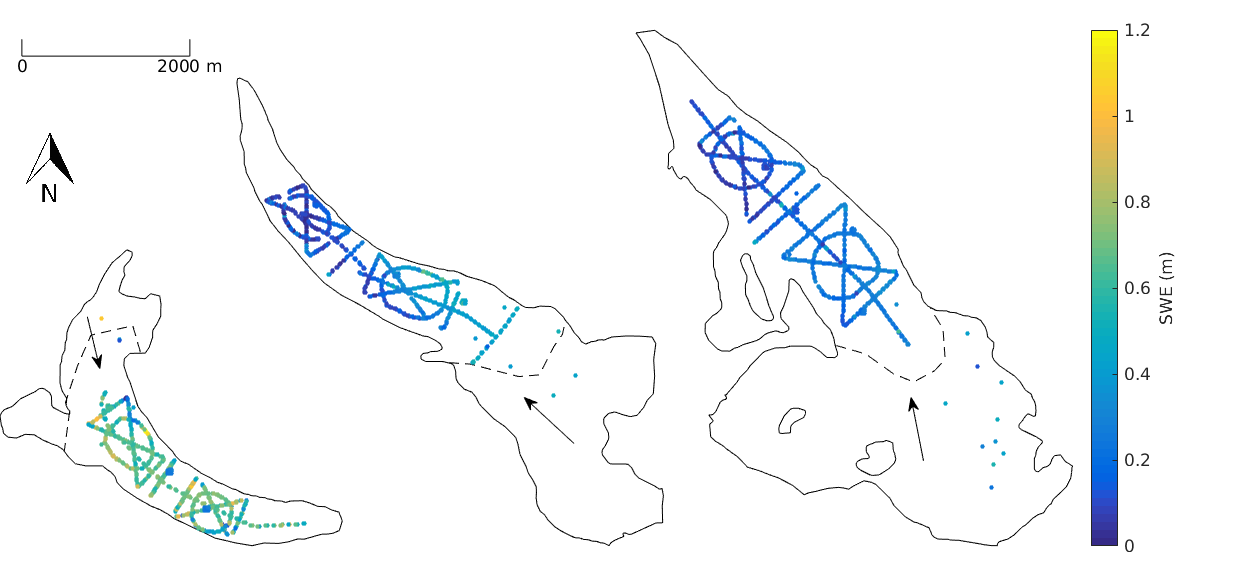
\includegraphics[width =\textwidth]{SWEmap_opt9.png}\\
	\caption{Estimated snow water equivalent (SWE) at measurement locations. Density was calculated using inverse distance weighting using all snowpit-derived densities (F4). Arrow shows ice flow direction.}
	\label{fig:SWEmap_F4}
\end{figure}


\end{document}